
\documentclass[10pt,openany,a4paper]{article}
\usepackage{tikz, pgfplots, tkz-euclide,calc}
\usetikzlibrary{patterns,shapes.arrows,calc}
\usepackage{fancyhdr}
\usepackage{enumerate,enumitem}
\usepackage{cancel}
\usepackage{varwidth}

% TAMBAHKAN PACKAGE SENDIRI KALAU KURANG

\usepackage{geometry}
\geometry{
	left = 22mm,
	right = 22mm,
	top = 25mm,
	bottom = 25mm,
}
\usepackage{graphicx}
\usepackage{subcaption}
\usepackage{soul}
\usepackage{hyperref}
\usepackage{float}
\usepackage{setspace}
\usepackage{afterpage}
\usepackage{xcolor}
\usepackage[nosectionbib]{apacite}
\usepackage{lmodern}
\usepackage{mathtools}
\usepackage{upgreek}
\usepackage{siunitx}
% \usepackage{fontawesome5}
\usepackage{fontawesome6}
\usepackage{physics}
\usepackage{pdfpages}
\usepackage{hyperref}
\renewcommand{\baselinestretch}{1.3}
\usepackage{multicol}
\usepackage{hyperref,ragged2e,amsmath,multicol,gensymb,setspace,
fancyhdr,amsfonts,tikz,pgfplots,nccmath,enumerate,verbatim,amsthm,physics}
\usepgfplotslibrary{polar,fillbetween}
% Disable tikz externalization to avoid requiring -shell-escape
\usepgfplotslibrary{external}
\tikzexternalize[prefix=tikz/]
\tikzset{reuse path/.code={\pgfsyssoftpath@setcurrentpath{#1}}}
\usetikzlibrary{shapes.geometric,arrows}
\newcommand\mylog[1]{\mathop{{}^{#1}\mathrm{log}}}
\pgfplotsset{compat=1.15}
\pgfplotsset{my style/.append style={axis x line=middle, axis y line=
middle, xlabel={$x$}, ylabel={$y$}, axis equal }}
\usepackage{etoolbox}
% remove stray \makeatother
\newtheorem{defn}{Definisi}[section]
\newtheorem{teo}[defn]{Teorema}
\newtheorem{thm}{Teorema}[section]
\newtheorem{lemma}{Lemma}
\newtheorem{lemmas}[defn]{Lemma}
\newtheorem{cor}[defn]{Akibat}
\newtheorem{asumsi}[defn]{Asumsi}
\theoremstyle{definition}
\newtheorem{con}{Contoh}[section]
\theoremstyle{definition}
\theoremstyle{plain}
\newtheorem{prop}{Proposisi}[section]
\renewcommand{\proofname}{Bukti}
\renewcommand{\thethm}{\arabic{chapter}.\arabic{thm}}

\newcommand{\normlp}[1]{\left\|#1\right\|_{L^p_{\lambda}(0,T;H)}}% Fungsi norm (||x||)
\newcommand{\R}{\mathbb{R}}
\renewcommand{\natural}{\mathbb{N}}
\newcommand{\Xpl}{X^R_{p,\lambda}}
\newcommand{\Xpls}{X^R_{p,\lambda^*}}
\newcommand{\qpl}{q^R_{p,\lambda}}
\newcommand{\qpls}{q^R_{p,\lambda^*}}
\pagestyle{fancy}
\fancyhf{}
\lhead{Halaman \thepage}
% \cfoot{\faXTwitter\ \href{https://x.com/ahmadzakiyudin_/}{@ahmadzakiyudin\_} | \faInstagram\ \href{https://instagram.com/ahmadzakiyudin_/}{@ahmadzakiyudin\_} | \faTiktok\ \href{https://tiktok.com/@ahmathz/}{@ahmathz}}
% \rhead{Pembahasan Soal ETS \\ Kalkulus 1 ITS 2025/2026}
\hypersetup{
    colorlinks=true,
    linkcolor=blue,
    filecolor=blue,      
    urlcolor=blue,
}
\newenvironment{jawab}[2][tes]{
% \fbox{\begin{minipage}{14.65cm}
\textbf{Kata kunci materi:} #1.\\
\textbf{Penyelesaian:} #2
% \end{minipage}}
}{}

\newenvironment{jawab2}[2][tes]{
\fbox{\begin{minipage}{14.65cm}
 #2
\end{minipage}}}{}

\newenvironment{jawaban}[2][tes]{
\colorlet{oldcolor}{.}
        \color{red}
        \setlength{\fboxrule}{1pt}\boxed{\color{oldcolor}#2}\color{oldcolor}.
}{}

\newenvironment{jawaban2}[2][tes]{
\colorlet{oldcolor}{.}
        \color{red}
        \setlength{\fboxrule}{1pt}\fbox{\color{oldcolor}#2}\color{oldcolor}.
}{}

\newenvironment{penting}[2][tes]{
\colorlet{oldcolor}{.}
\color{blue}
\fbox{\color{oldcolor}#2}\color{oldcolor}
}{}

\begin{document}
% \begin{titlepage}
%     \vspace*{\fill}
%     \begin{center}
%       \Huge {PEMBAHASAN SOAL EAS \\ KALKULUS II \\ TAHUN 2024/2025}\\[0.4 cm]
%       \huge {Ahmad Hisbu Zakiyudin}\\[0.2 cm]
%       \Large {(\href{https://instagram.com/ahmadzakiyudin_/}{@ahmadzakiyudin\_})}
%     \end{center}
%     \vspace*{\fill}
%   \end{titlepage}
% !TEX root = ../../BookTemplate.tex
%%%%%%%%%%%%%%%%%%%%%%%%%%%%%%%%%%%%%%%%%%%%%%%%%%%%%%%%%%%%%%%%%%%%%%%%%%%%%%%%%%
% \begin{titlepage}
%     \raggedleft	
% 	\hspace{.025\textwidth}
% 	\parbox[b]{\textwidth}{
%     \vspace{1.5cm}
% 		{\Huge\bfseries Pembahasan Soal EAS}                \\[20pt]
% 		{\huge\textit\ Kalkulus II}\\ \\[10pt]
%         {\Large\textsc{Tahun 2024/2025}}}
% \vfill
% \rule{1pt}{.14\textheight}
% \hspace{.025\textwidth}
%     \raisebox{10pt}{\parbox[b]{.95\textwidth}{ 
%         {\Large\textsc{Ahmad Hisbu Zakiyudin}}              \\[10pt]
%         \large{\href{https://instagram.com/ahmadzakiyudin_/}{@ahmadzakiyudin\_}}               \\[25pt]
%         {\large 5 Juni 2026}}}
% \end{titlepage}
\begin{titlepage}
	\centering % Center everything on the title page
	% \scshape % Use small caps for all text on the title page
	\vspace*{1.5\baselineskip} % White space at the top of the page
% ===================
%	Title Section 	
% ===================

	\rule{13cm}{1.6pt}\vspace*{-\baselineskip}\vspace*{2pt} % Thick horizontal rule
	\rule{13cm}{0.4pt} % Thin horizontal rule
	
		\vspace{0.75\baselineskip} % Whitespace above the title
% ========== Title ===============	
	{	\Huge Pembahasan Soal ETS\\ 
			\vspace{4mm}
		Kalkulus 1 \\ \vspace{2mm} \huge{Tahun 2025/2026}\\	}
% ======================================
		\vspace{0.75\baselineskip} % Whitespace below the title
	\rule{13cm}{0.4pt}\vspace*{-\baselineskip}\vspace{3.2pt} % Thin horizontal rule
	\rule{13cm}{1.6pt} % Thick horizontal rule
	
		\vspace{1.75\baselineskip} % Whitespace after the title block
% =================
%	Information	
% =================
{\large Oleh: Ahmad Hisbu Zakiyudin}
	% {\large Oleh: Ahmad Hisbu Zakiyudin \\
	% 	\vspace*{1.2\baselineskip}
	% \href{https://instagram.com/ahmadzakiyudin_/}{@ahmadzakiyudin\_}} \\
	\vfill
	\vspace{1mm}
\huge{Selamat Belajar!}
\end{titlepage}
\makeatletter
\setlength\fboxsep{3pt}
% ensure enough header height for fancyhdr
\setlength{\headheight}{24pt}
 \begin{center}
	{\underline{\textbf{\MakeUppercase{Soal dan Pembahasan ETS Kalkulus 1 Tahun 2025/2026}}}}
    \end{center}

    \begin{center}
	\begin{tabular}{lcl}
		Mata kuliah/SKS & : & Kalkulus 1 ( SM234101 ) / 3 SKS\\
		Hari, Tanggal & : & Senin, 13 Oktober 2025\\
		Waktu & : & 07.00 - 08.40 / 100 menit\\
		Sifat & : & Tertutup\\
		Kelas & : & 40-49, 62-66\\
  ~
	\end{tabular}
    
    \noindent\rule{\textwidth}{2.pt}
        \end{center}
    \begin{enumerate}
     \item Dapatkan semua nilai \(x\) yang memenuhi pertidaksamaan
    \(
        \dfrac{2x + 1}{3x - 6} < \dfrac{1}{2}.
    \)\\
\begin{jawab}[pertidaksamaan rasional, pecahan, garis bilangan, notasi interval]{
        ~\\
        Untuk menyelesaikan pertidaksamaan rasional, pastikan ruas kanan sudah bernilai nol. Dengan mengurangkan \(\frac{1}{2}\) dari kedua ruas, didapatkan
        \[
        \frac{2x + 1}{3x - 6} - \frac{1}{2} < 0
        \]
        Selanjutnya, dengan menyamakan penyebut dan menyederhanakan bentuknya, diperoleh
        \begin{align}
            \frac{2(2x+1)-(3x-6)}{2(3x-6)} &< 0\nonumber\\
             \frac{4x + 2 - 3x + 6}{2(3x - 6)} &< 0\nonumber \\
             \frac{x + 8}{2(3x - 6)} &< 0 \label{ineq:soal1}
        \end{align}
        Didapatkan pembuat nol dari faktor-faktornya adalah 
        \begin{align*}
            x+8 = 0 \quad &\vee\quad  3x - 6 = 0\\
            \colorlet{oldcolor}{.}
        \color{blue}
        \setlength{\fboxrule}{1pt} \boxed{\color{oldcolor}x=-8}\color{oldcolor}
         \quad &\vee\quad \colorlet{oldcolor}{.}
        \color{blue}
        \setlength{\fboxrule}{1pt} \boxed{\color{oldcolor}x=2}\color{oldcolor}
        \end{align*}
        Selanjutnya, dibuat garis bilangan dan dilakukan uji titik pada ekspresi \eqref{ineq:soal1} sebagai berikut
        \begin{itemize}
            \item Untuk \(x < -8\), misalkan \(x = -10\):
            \[
            \frac{-10 + 8}{2(3(-10) - 6)} = \frac{-2}{2(-30 - 6)} = \frac{-2}{2(-36)} = \frac{-2}{-72} > 0
            \]
            \item Untuk \(-8 < x < 2\), misalkan \(x = 0\):
            \[
            \frac{0 + 8}{2(3(0) - 6)} = \frac{8}{2(-6)} = \frac{8}{-12} < 0
            \]
            \item Untuk \(x > 2\), misalkan \(x = 5\):
            \[
            \frac{5 + 8}{2(3(5) - 6)} = \frac{13}{2(15 - 6)} = \frac{13}{2(9)} > 0
            \]
        \end{itemize}
        \begin{center}
           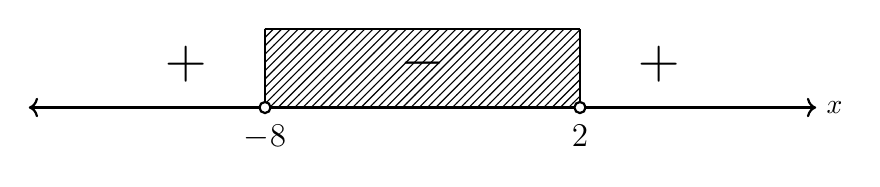
\begin{tikzpicture}

    % Garis bilangan
    \draw[thick,<->] (-5,0) -- (5,0) node[right] {$x$};

    % Arsiran daerah negatif
    \fill[pattern=north east lines] (-2,0) rectangle (2,1);

    % Label titik
    \draw (-2,-0.1) node[below] {\large{$-8$}};
    \draw (2,-0.1) node[below] {\large{$2$}};

    % Tanda batas dan bagian atas
    \draw[thick] (-2,0) -- (-2,1);
    \draw[thick] (2,0) -- (2,1);
    \draw[thick] (-2,1) -- (2,1);

    % Tanda positif-negatif
    \draw (0,0.2) node[above] {\huge{$-$}};
    \draw (3,0.2) node[above] {\huge{$+$}};
    \draw (-3,0.2) node[above] {\huge{$+$}};

    % Titik terbuka
    \draw[fill=white, thick] (-2,0) circle (2pt);
    \draw[fill=white, thick] (2,0) circle (2pt);

\end{tikzpicture}
        \end{center}
        Karena yang diminta adalah nilai \(x\) yang membuat pertidaksamaan \eqref{ineq:soal1} kurang dari nol, maka solusi dari pertidaksamaan tersebut adalah \(-8 < x < 2\). Dalam notasi interval, solusi tersebut dapat ditulis sebagai $\colorlet{oldcolor}{.}
        \color{red}
        \setlength{\fboxrule}{1pt} \boxed{\color{oldcolor}(-8, 2)}\color{oldcolor}$.}
    \end{jawab}
    \item Diberikan fungsi \(f(x) = \frac{1}{x-1}\) dan \(g(x) = 2 - \sqrt{x}\).
    \begin{enumerate}
        \item Tentukan domain dari fungsi \(f\) dan \(g\).
        \item Dapatkan fungsi \((f \circ g)(x)\) beserta domainnya.
    \end{enumerate}
    \begin{jawab}[domain fungsi, fungsi komposisi, domain fungsi komposisi]{
        \begin{enumerate}
            \item Diperhatikan bahwa $f(x)$ merupakan fungsi rasional, sehingga domainnya adalah semua bilangan real kecuali nilai yang membuat penyebutnya sama dengan nol, yaitu $x-1\neq 0$. Jadi
            \[
            \colorlet{oldcolor}{.}
        \color{red}
        \setlength{\fboxrule}{1pt} \boxed{\color{oldcolor}D(f)=\{x \in \mathbb{R} : x \neq 1\}}\color{oldcolor}.
            \]
            Selanjutnya, diperhatikan bahwa $g(x)$ memuat akar kuadrat, sehingga domainnya adalah semua bilangan real yang membuat ekspresi di dalam akar kuadrat tak negatif. Jadi 
            \[
            \colorlet{oldcolor}{.}
        \color{red}
        \setlength{\fboxrule}{1pt} \boxed{\color{oldcolor}D(g)=\{x \in \mathbb{R} : x \geq 0\}}\color{oldcolor}.
            \]
            \item Diperhatikan bahwa 
            \begin{align*}
                (f\circ g)(x) = f(g(x)) = f(2 - \sqrt{x}) = \frac{1}{(2 - \sqrt{x}) - 1} = 
                \colorlet{oldcolor}{.}
        \color{red}
        \setlength{\fboxrule}{1pt} \boxed{\color{oldcolor}\frac{1}{1 - \sqrt{x}}}\color{oldcolor}
            \end{align*}
            Domain dari fungsi komposisi $f\circ g$ adalah semua nilai $x$ pada domain $g$ sehingga nilai dari $g(x)$ berada pada domain $f$, yang dapat dirumuskan sebagai 
            \begin{align*}
                \colorlet{oldcolor}{.}
        \color{blue}
        \setlength{\fboxrule}{1pt} \boxed{\color{oldcolor}D(f\circ g) = \{x \in D(g) : g(x) \in D(f)\} = \{x \in [0, \infty) : 2 - \sqrt{x} \neq 1\}}\color{oldcolor}.
            \end{align*}
            Karena $2 - \sqrt{x} = 1$ jika dan hanya jika $\sqrt{x} = 1$, yang berarti $x = 1$, didapatkan
            \begin{align*}
                \colorlet{oldcolor}{.}
        \color{red}
        \setlength{\fboxrule}{1pt} \boxed{\color{oldcolor}D(f\circ g) = [0, \infty) \setminus \{1\} = [0, 1) \cup (1, \infty)}\color{oldcolor}.
            \end{align*}
        \end{enumerate}
    }
        
    \end{jawab}

    \item Diberikan fungsi \(f(x) = \begin{cases} \frac{x^3-8}{2x-4}, & x \neq 2 \\ k, & x=2 \end{cases}\).
    \begin{enumerate}
        \item Tentukan nilai \(k\) sehingga \(f(x)\) kontinu di \(x = 2\).
        \item Berdasarkan hasil dari (a), nyatakan \(f(x)\) sebagai polinomial.
    \end{enumerate}
    \begin{jawab}[fungsi kontinu, limit, polinomial]{
        \begin{enumerate}
            \item Ingat kembali syarat fungsi kontinu di suatu titik \(x = a\) adalah
            \begin{enumerate}
                \item \(f(a)\) terdefinisi
                \item \(\displaystyle \lim_{x \to a} f(x)\) ada, yaitu $\displaystyle \lim_{x \to a^-} f(x) = \lim_{x \to a^+} f(x)$
                \item \(\displaystyle\lim_{x \to a} f(x) = f(a)\)
            \end{enumerate} 
            Diperhatikan bahwa untuk \(x = 2\), \(\colorlet{oldcolor}{.}
        \color{blue}
        \setlength{\fboxrule}{1pt} \boxed{\color{oldcolor}f(2) = k~\text{terdefinisi}}\color{oldcolor}\). Karena limit di $x=2$ artinya nilai fungsi di sekitar $x=2$ tetapi $x\neq 2$, didapatkan limitnya adalah
            \begin{align*}
            \lim_{x \to 2} f(x) = \lim_{x \to 2} \frac{x^3 - 8}{2x - 4} = \lim_{x \to 2} \frac{(x-2)(x^2 + 2x + 4)}{2(x-2)} = \lim_{x \to 2} \frac{x^2 + 2x + 4}{2} = \frac{4 + 4 + 4}{2} = \colorlet{oldcolor}{.}
        \color{blue}
        \setlength{\fboxrule}{1pt} \boxed{\color{oldcolor}6}\color{oldcolor}.
            \end{align*}
            Selanjutnya, untuk syarat ketiga, haruslah $\displaystyle \colorlet{oldcolor}{.}
        \color{blue}
        \setlength{\fboxrule}{1pt} \boxed{\color{oldcolor}\lim_{x \to 2} f(x) = f(2)}\color{oldcolor}$, sehingga diperoleh $\colorlet{oldcolor}{.}
        \color{red}
        \setlength{\fboxrule}{1pt} \boxed{\color{oldcolor}k=6}\color{oldcolor}$.
        \item Diperhatikan bahwa untuk $x\neq 2$, berlaku 
        \begin{align*}
            f(x) = \frac{x^3 - 8}{2x - 4} = \frac{(x-2)(x^2 + 2x + 4)}{2(x-2)} = \frac{x^2 + 2x + 4}{2} = \frac{1}{2}x^2 + x + 2.
        \end{align*}
        Berdasarkan hasil dari (a), diperoleh bahwa \(f(x)\) kontinu di \(x=2\) jika \(k=6\). Dengan demikian, fungsi \(f(x)\) dapat dinyatakan sebagai polinomial
        \begin{align*}
            \colorlet{oldcolor}{.}
        \color{red}
        \setlength{\fboxrule}{1pt} \boxed{\color{oldcolor}f(x) = \frac{1}{2}x^2 + x + 2}\color{oldcolor}.
        \end{align*}
        \end{enumerate}
    }
        
    \end{jawab}

    \item Diberikan fungsi implisit \(3x^2 + y^2 - 2xy + y - x = 6\). Tentukan \(\frac{dy}{dx}\) di titik \((0,-3)\).\\
    \begin{jawab}[diferensiasi implisit, turunan, aturan perkalian, aturan rantai]{~\\
        Diperoleh turunan implisit dari fungsi tersebut dengan menurunkan kedua ruas terhadap \(x\):
        \begin{align*}
            \frac{d}{dx}(3x^2 + y^2 - 2xy + y - x) &= \frac{d}{dx}(6)\\
            \frac{d}{dx}(3x^2) + \frac{d}{dx}(y^2) - \frac{d}{dx}(2xy) + \frac{d}{dx}(y) - \frac{d}{dx}(x) &= 0
        \end{align*}
        Untuk suku-suku yang tidak mengandung \(y\), turunan terhadap \(x\) dapat dihitung langsung. Untuk suku-suku yang mengandung \(y\), digunakan aturan rantai dan aturan perkalian. Misalkan $\colorlet{oldcolor}{.}
        \color{blue}
        \setlength{\fboxrule}{1pt} \boxed{\color{oldcolor}u=y^2}\color{oldcolor}$, maka dengan aturan rantai diperoleh
        \begin{align*}
            \colorlet{oldcolor}{.}
        \color{blue}
        \setlength{\fboxrule}{1pt} \boxed{\color{oldcolor}\frac{du}{dx} = \frac{du}{dy}\frac{dy}{dx} = 2y\frac{dy}{dx}}\color{oldcolor}
        \end{align*}
        Misalkan $\colorlet{oldcolor}{.}
        \color{blue}
        \setlength{\fboxrule}{1pt} \boxed{\color{oldcolor}u=2x}\color{oldcolor}$ dan $\colorlet{oldcolor}{.}
        \color{blue}
        \setlength{\fboxrule}{1pt}\boxed{\color{oldcolor}v=y}\color{oldcolor}$, maka dengan aturan perkalian diperoleh
        \begin{align*}
        \frac{d}{dx}(2xy)=u'v+v'u=y\frac{d}{dx}(2x) + x\frac{dy}{dx}= \colorlet{oldcolor}{.}
        \color{blue}
        \setlength{\fboxrule}{1pt} \boxed{\color{oldcolor}2\left(y + x\frac{dy}{dx}\right)}\color{oldcolor}.
        \end{align*}
        Dengan demikian, diperoleh
        \begin{align*}
            6x + 2y\frac{dy}{dx} - 2\left(y + x\frac{dy}{dx}\right) + \frac{dy}{dx} - 1 &= 0\\
            2y\frac{dy}{dx}  - 2x\frac{dy}{dx} + \frac{dy}{dx}  &= 1+2y-6x\\
            (2y - 2x + 1)\frac{dy}{dx} + (6x - 2y - 1) &= 0\\
            \frac{dy}{dx} &=
            \colorlet{oldcolor}{.}
        \color{red}
        \setlength{\fboxrule}{1pt} \boxed{\color{oldcolor}\frac{1+2y-6x}{(2y - 2x + 1)}}\color{oldcolor}
        \end{align*}
        Selanjutnya, substitusi titik \((0,-3)\) ke dalam persamaan turunan:
        \begin{align*}
            \frac{dy}{dx}\bigg|_{(0,-3)} &= \frac{1+2(-3)-6(0)}{(2(-3) - 2(0) + 1)}= \frac{1-6}{-6 + 1}= \frac{-5}{-5}= \colorlet{oldcolor}{.}
        \color{red}
        \setlength{\fboxrule}{1pt} \boxed{\color{oldcolor}1}\color{oldcolor}.
        \end{align*}
    }
        
    \end{jawab}

    \item Diketahui garis \(g_1: y = -x + 6\) dan garis \(g_2: y = 2x\).
    \begin{enumerate}
        \item Tentukan titik potong kedua garis \(g_1\) dan \(g_2\).
        \item Tentukan titik potong \(g_1\) dengan garis \(x = 1\).
        \item Tentukan pula titik potong \(g_2\) dengan garis \(x = 1\). Gambarkan sketsa ketiga garis \(g_1\), \(g_2\), dan garis \(x = 1\). Hitung luas segitiga yang dibentuk ketiga garis tersebut.
    \end{enumerate}
    \begin{jawab}[persamaan garis,titik potong garis, luas segitiga]{
        \begin{enumerate}
            \item Untuk menentukan titik potong kedua garis, kita samakan persamaan kedua garis, yaitu $-x+6=2x$, sehingga $6=3x$, dan diperoleh $x=2$. Selanjutnya, substitusi \(x = 2\) ke dalam salah satu persamaan garis, misalkan \(g_2\), diperoleh $y=2(2)=4$. Jadi titik potong kedua garis adalah \(\colorlet{oldcolor}{.}
        \color{red}
        \setlength{\fboxrule}{1pt} \boxed{\color{oldcolor}(2,4)}\color{oldcolor}\), misalkan sebagai titik $A$
            \item Untuk menentukan titik potong \(g_1\) dengan garis \(x = 1\), substitusi \(x = 1\) ke dalam persamaan \(g_1\), yaitu $y = -1 + 6 = 5$. Jadi titik potong \(g_1\) dengan garis \(x = 1\) adalah \(\colorlet{oldcolor}{.}
        \color{red}
        \setlength{\fboxrule}{1pt} \boxed{\color{oldcolor}(1,5)}\color{oldcolor}\). Misalkan titik potong tersebut sebagai titik $B$
            \item Untuk menentukan titik potong \(g_2\) dengan garis \(x = 1\), substitusi \(x = 1\) ke dalam persamaan \(g_2\), yaitu $y = 2(1) = 2$. Jadi titik potong \(g_2\) dengan garis \(x = 1\) adalah \(\colorlet{oldcolor}{.}
        \color{red}
        \setlength{\fboxrule}{1pt} \boxed{\color{oldcolor}(1,2)}\color{oldcolor}\). Misalkan titik potong tersebut sebagai titik $C$.\\
            Dengan melakukan plot titik-titik potong tersebut dan menarik garis di antara dua titik potong, didapatkan sketsa dari ketiga garis dan segitiga tersebut adalah sebagai berikut
            \begin{center}
                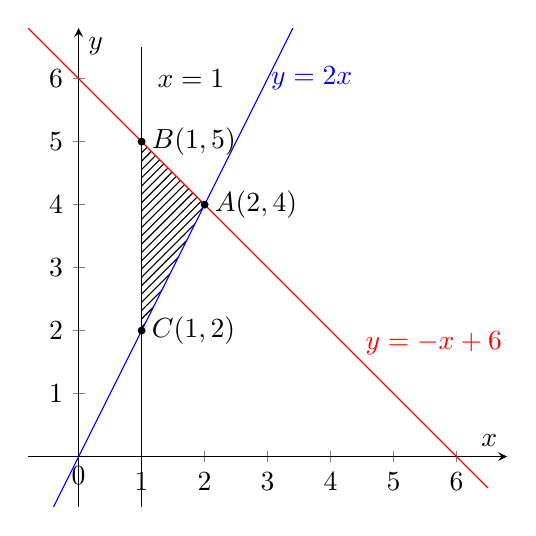
\begin{tikzpicture}
                   \begin{axis}[
x =0.8 cm, y=0.8 cm,
axis lines=middle,
xmin=-0.8,xmax=6.8,
ymin=-0.8,ymax=6.8,
xtick distance=1,
ytick distance=1,
xlabel=$x$,
ylabel=$y$
]
\addplot[opacity=0, domain=1:2, name path=A] {2*x};
\addplot[opacity=0, domain=1:2, name path=B] {-x+6};
% Kurva y = sqrt(x)
\addplot [red,domain=-1:6.5, samples=1000] {-x+6};

% Garis y = 2
\addplot [blue,domain=-1:6.5, samples=1000] {2*x};

% Daerah arsiran
\addplot[pattern=north east lines] fill between[of=A and B, soft clip={domain=1:2}];


% Garis x = 0
\draw (1,-1.5) -- (1,6.5);

% Sumbu putar x = -2
\draw[dashed] (-2,-0.5) -- (-2,3);
\draw (-2.2,2.7) node{$x=-2$};
\draw (1.1,6) node[right]{$x=1$};

% Label kurva
\draw[blue] (3.7,6) node{$y=2x$};
\draw[red] (4.4,1.8) node[right] {$y=-x+6$};
\draw[fill=black, thick] (2,4) circle (1pt) node[right] {$A(2,4)$};
\draw[fill=black, thick] (1,5) circle (1pt) node[right] {$B(1,5)$};
\draw[fill=black, thick] (1,2) circle (1pt) node[right] {$C(1,2)$};
% Label x=0
\draw (0,-0.3) node{$0$};

\end{axis}
                \end{tikzpicture}
            \end{center}
            Pandang garis $BC$ sebagai alas segitiga, sehingga panjang alasnya adalah $|5-2|=\colorlet{oldcolor}{.}
        \color{blue}
        \setlength{\fboxrule}{1pt} \boxed{\color{oldcolor}3}\color{oldcolor}$. Selanjutnya, pandang garis $A$ sebagai titik puncak segitiga, sehingga tinggi segitiga adalah jarak dari titik $A$ ke garis $BC$, yaitu jarak dari titik $(2,4)$ ke garis $x=1$, yang panjangnya adalah $|2-1|=\colorlet{oldcolor}{.}
        \color{blue}
        \setlength{\fboxrule}{1pt} \boxed{\color{oldcolor}1}\color{oldcolor}$. Dengan demikian, luas segitiga tersebut adalah
            \[
            L = \frac{1}{2} \times \text{alas} \times \text{tinggi} = \frac{1}{2} \times 3 \times 1 = \colorlet{oldcolor}{.}
        \color{red}
        \setlength{\fboxrule}{1pt} \boxed{\color{oldcolor}\frac{3}{2}}\color{oldcolor}.
            \]
        \end{enumerate}
    }
    \end{jawab}
\end{enumerate}
\newpage
 \begin{center}
	{\underline{\textbf{\MakeUppercase{Soal dan Pembahasan ETS Kalkulus 1 Tahun 2025/2026}}}}
    \end{center}

    \begin{center}
	\begin{tabular}{lcl}
		Course / Credit & : & Kalkulus 1 ( SM234101 ) / 3 SKS\\
		Day, Date & : & Monday, 13 October 2025\\
		Time / Exam Time & : & 09.00 - 10.40 / 100 menit\\
		Type & : & Tertutup\\
		Class & : & 1, 4, 67, 70, 71\\
  ~
	\end{tabular}
    
    \noindent\rule{\textwidth}{2.pt}
        \end{center}
\begin{enumerate}
           \item Solve the following inequality.
    \( \frac{x^2 - x - 12}{x^2 - 2x - 3} \ge 0. \)\\
    \begin{jawab}[pertidaksamaan rasional, persamaan kuadrat, notasi interval]{~\\
    Karena ruas kanan pertidaksamaan sudah bernilai nol, maka kita bisa langsung memfaktorkan pembilang dan penyebut di ruas kiri. Diperoleh
    \begin{align*}
        \frac{x^2 - x - 12}{x^2 - 2x - 3} &= \frac{(x-4)(x+3)}{(x-3)(x+1)} \ge 0
    \end{align*}
    Selanjutnya, kita tentukan pembuat nol dari faktor-faktor tersebut, yaitu
    \begin{align*}
        x-4 = 0 \quad &\vee\quad x+3 = 0 \quad \vee\quad x-3 = 0 \quad \vee\quad x+1 = 0\\
        \colorlet{oldcolor}{.}
        \color{blue}
        \setlength{\fboxrule}{1pt} \boxed{\color{oldcolor}x=4}\color{oldcolor} \quad &\vee\quad \colorlet{oldcolor}{.}
        \color{blue}
        \setlength{\fboxrule}{1pt} \boxed{\color{oldcolor}x=-3}\color{oldcolor} \quad \vee\quad \colorlet{oldcolor}{.}
        \color{blue}
        \setlength{\fboxrule}{1pt} \boxed{\color{oldcolor}x=3}\color{oldcolor} \quad \vee\quad \colorlet{oldcolor}{.}
        \color{blue}
        \setlength{\fboxrule}{1pt} \boxed{\color{oldcolor}x=-1}\color{oldcolor}
    \end{align*}
    Selanjutnya, kita buat garis bilangan dan lakukan uji titik pada ekspresi \(\frac{(x-4)(x+3)}{(x-3)(x+1)}\) sebagai berikut
    \begin{itemize}
        \item Untuk \(x < -3\), misalkan \(x = -4\):
        \[
        \frac{(-4-4)(-4+3)}{(-4-3)(-4+1)} = \frac{(-8)(-1)}{(-7)(-3)} = \frac{8}{21} > 0
        \]
        \item Untuk \(-3 < x < -1\), misalkan \(x = -2\):
        \[
        \frac{(-2-4)(-2+3)}{(-2-3)(-2+1)} = \frac{(-6)(1)}{(-5)(-1)} = \frac{-6}{5} < 0
        \]
        \item Untuk \(-1 < x < 3\), misalkan \(x = 0\):
        \[
        \frac{(0-4)(0+3)}{(0-3)(0+1)} = \frac{(-4)(3)}{(-3)(1)} = \frac{-12}{-3} = 4 > 0
        \]
        \item Untuk \(3 < x < 4\), misalkan \(x = 3.5\):
        \[
        \frac{(3.5-4)(3.5+3)}{(3.5-3)(3.5+1)} = \frac{(-0.5)(6.5)}{(0.5)(4.5)} = \frac{-3.25}{2.25} < 0
        \]
        \item Untuk \(x > 4\), misalkan \(x = 5\):
        \[
        \frac{(5-4)(5+3)}{(5-3)(5+1)} = \frac{(1)(8)}{(2)(6)} = \frac{8}{12} = \frac{2}{3} > 0
        \]
    \end{itemize}
    Jadi solusi dari pertidaksamaan tersebut adalah \(x \in (-\infty, -3] \cup [-1, 3) \cup [4, \infty)\). Dalam notasi interval, solusi tersebut dapat ditulis sebagai $\colorlet{oldcolor}{.}
        \color{red}
        \setlength{\fboxrule}{1pt} \boxed{\color{oldcolor}(-\infty, -3] \cup [-1, 3) \cup [4, \infty)}\color{oldcolor}$.
    }
        
    \end{jawab}

    \item Given a function \(f(x) = 2 - \sqrt{x}\) and \(g(x) = \frac{1}{x-1}\). Determine:
    \begin{enumerate}
        \item[a)] The domain of function \(f\) and \(g\);
        \item[b)] Function \((f \circ g)(x)\) and its domain.
    \end{enumerate}
    \begin{jawab}[domain fungsi, fungsi komposisi, domain fungsi komposisi]{
        \begin{enumerate}
            \item Diperhatikan bahwa $f(x)$ memuat akar kuadrat, sehingga domainnya adalah semua bilangan real yang membuat ekspresi di dalam akar kuadrat tak negatif. Jadi 
            \begin{align*}
                \colorlet{oldcolor}{.}
        \color{red}
        \setlength{\fboxrule}{1pt} \boxed{\color{oldcolor}D(f)=\{x \in \mathbb{R} : x \geq 0\}}\color{oldcolor}.
            \end{align*}
            Selanjutnya, diperhatikan bahwa $g(x)$ merupakan fungsi rasional, sehingga domainnya adalah semua bilangan real kecuali nilai yang membuat penyebutnya sama dengan nol, yaitu $x-1\neq 0$. Jadi
            \begin{align*}
                \colorlet{oldcolor}{.}
        \color{red}
        \setlength{\fboxrule}{1pt} \boxed{\color{oldcolor}D(g)=\{x \in \mathbb{R} : x \neq 1\}}\color{oldcolor}.
            \end{align*}
            \item Diperhatikan bahwa 
            \begin{align*}
                (f\circ g)(x) = f(g(x)) = f\left(\frac{1}{x-1}\right) = 2 - \sqrt{\frac{1}{x-1}} = 2 - \frac{1}{\sqrt{x-1}}
            \end{align*}
            Domain dari fungsi komposisi $f\circ g$ adalah semua nilai $x$ pada domain $g$ sehingga nilai dari $g(x)$ berada pada domain $f$, yang dapat dirumuskan sebagai 
            \begin{align*}
                \colorlet{oldcolor}{.}
        \color{blue}
        \setlength{\fboxrule}{1pt} \boxed{\color{oldcolor}D(f\circ g) = \{x \in D(g) : g(x) \in D(f)\} = \left\{x \neq 1 : \frac{1}{x-1} \geq 0\right\}}\color{oldcolor}.
            \end{align*}
            Karena $\frac{1}{x-1} \geq 0$ jika dan hanya jika $x-1 > 0$, yang berarti $x > 1$, didapatkan
            \begin{align*}
                \colorlet{oldcolor}{.}
        \color{red}
        \setlength{\fboxrule}{1pt} \boxed{\color{oldcolor}D(f\circ g) = (1, \infty)}\color{oldcolor}.
            \end{align*}
        \end{enumerate}
    }
        
    \end{jawab}

    \item Write the derivative formula of \(\frac{f}{g}\), that is \(\frac{d}{dx}\left(\frac{f(x)}{g(x)}\right)\). \\
    Then, find the derivative of \(\frac{f}{g}\) given that \(f(x) = 2x^2 + 3x - 2\) and \(g(x) = x - 1\) for \(x \neq 1\).
    \begin{jawab}[turunan, aturan pembagian]{
        Ingat kembali aturan turunan untuk pembagian fungsi, yaitu
        \[
        \frac{d}{dx}\left(\frac{f(x)}{g(x)}\right) = \frac{f'(x)g(x) - f(x)g'(x)}{(g(x))^2}
        \]
        Selanjutnya, kita hitung turunan dari \(f(x)\) dan \(g(x)\):
        \begin{align*}
            f'(x) &= \frac{d}{dx}(2x^2 + 3x - 2) = 4x + 3\\
            g'(x) &= \frac{d}{dx}(x - 1) = 1
        \end{align*}
        Dengan demikian, turunan dari \(\frac{f}{g}\) adalah
        \begin{align*}
            \frac{d}{dx}\left(\frac{f(x)}{g(x)}\right) &= \frac{(4x + 3)(x - 1) - (2x^2 + 3x - 2)(1)}{(x - 1)^2}\\
            &= \frac{(4x^2 - 4x + 3x - 3) - (2x^2 + 3x - 2)}{(x - 1)^2}\\
            &= \frac{4x^2 - x - 3 - 2x^2 - 3x + 2}{(x - 1)^2}\\
            &= \frac{2x^2 - 4x - 1}{(x - 1)^2}
        \end{align*}
    }
        
    \end{jawab}

    \item Given \(f(x) = \begin{cases} \frac{x^3-8}{2x-4}, & x \neq 2 \\ 2k, & x=2 \end{cases}\).
    \begin{enumerate}
        \item[a.] Determine k such that \(f(x)\) continuous at \(x = 2\).
        \item[b.] Based on the result of a), rewrite \(f(x)\) as a polynomial.
    \end{enumerate}
    \begin{jawab}[fungsi kontinu, limit, polinomial]{
        \begin{enumerate}
            \item Ingat kembali syarat fungsi kontinu di suatu titik \(x = a\) adalah
            \begin{enumerate}
                \item \(f(a)\) terdefinisi
                \item \(\displaystyle \lim_{x \to a} f(x)\) ada, yaitu $\displaystyle \lim_{x \to a^-} f(x) = \lim_{x \to a^+} f(x)$
                \item \(\displaystyle\lim_{x \to a} f(x) = f(a)\)
            \end{enumerate} 
            Diperhatikan bahwa untuk \(x = 2\), $\colorlet{oldcolor}{.}
        \color{blue}
        \setlength{\fboxrule}{1pt} \boxed{\color{oldcolor}f(2) = 2k~\text{terdefinisi}}\color{oldcolor}$. Karena limit di $x=2$ artinya nilai fungsi di sekitar $x=2$ tetapi $x\neq 2$, didapatkan limitnya adalah
            \begin{align*}
            \lim_{x \to 2} f(x) = \lim_{x \to 2} \frac{x^3 - 8}{2x - 4} = \lim_{x \to 2} \frac{(x-2)(x^2 + 2x + 4)}{2(x-2)} = \lim_{x \to 2} \frac{x^2 + 2x + 4}{2} = 6
            \end{align*}
            Selanjutnya, untuk syarat ketiga, haruslah $\displaystyle\lim_{x \to 2} f(x) = f(2)$, sehingga diperoleh $6 = 2k$, dan didapatkan $\colorlet{oldcolor}{.}
        \color{red}
        \setlength{\fboxrule}{1pt} \boxed{\color{oldcolor}k=3}\color{oldcolor}$.
        \item Diperhatikan bahwa untuk $x\neq 2$, berlaku
        \begin{align*}
            f(x) = \frac{x^3 - 8}{2x - 4} = \frac{(x-2)(x^2 + 2x + 4)}{2(x-2)} = \frac{x^2 + 2x + 4}{2} = \frac{1}{2}x^2 + x + 2.
        \end{align*}
        Berdasarkan hasil dari (a), diperoleh bahwa \(f(x)\) kontinu di \(x=2\) jika \(k=3\). Dengan demikian, fungsi \(f(x)\) dapat dinyatakan sebagai polinomial
        \begin{align*}
            \colorlet{oldcolor}{.}
        \color{red}
        \setlength{\fboxrule}{1pt} \boxed{\color{oldcolor}f(x) = \frac{1}{2}x^2 + x + 2}\color{oldcolor}.
        \end{align*}
        \end{enumerate}
    }
    \end{jawab}

    \item Sketch the base curve \(x = y^2\). Based on that base curve, use translation to sketch the curve \(x = y^2 + 4y + 1\). (Explain the process).

        \end{enumerate}
               \newpage
 \begin{center}
	{\underline{\textbf{\MakeUppercase{Soal dan Pembahasan ETS Kalkulus 1 Tahun 2025/2026}}}}
    \end{center}

    \begin{center}
	\begin{tabular}{lcl}
		Mata kuliah/SKS & : & Kalkulus 1 ( SM234101 ) / 3 SKS\\
		Hari, Tanggal & : & Senin, 13 Oktober 2025\\
		Waktu & : & 11.00 - 12.40 / 100 menit\\
		Sifat & : & Tertutup\\
		Kelas & : & 17-22\\
  ~
	\end{tabular}
    
    \noindent\rule{\textwidth}{2.pt}
        \end{center}
\begin{enumerate}
    \item \begin{enumerate}
        \item Nyatakan pernyataan $\sqrt{(2x-1)^2}$ dalam bentuk nilai mutlak.
        \item Dapatkan semua nilai $x$ yang memenuhi persamaan $\sqrt{(2x-1)^2}=1-2x$.
    \end{enumerate}
    \begin{jawab}[definisi nilai mutlak, persamaan nilai mutlak]{
        \begin{enumerate}
            \item Ingat bahwa $\sqrt{x^2}=|x|$, sehingga diperoleh
            \begin{align*}
                \sqrt{(2x-1)^2} = |2x-1|
            \end{align*}
            \item Diperhatikan bahwa 
            \begin{align*}
                |2x-1| = 1-2x = -(2x-1)
            \end{align*}
            Kemudian, pertimbangkan definisi nilai mutlak, yaitu
            \begin{align*}
                |2x-1| = \begin{cases}
                    2x-1, & 2x-1 \geq 0\\
                    -(2x-1), & 2x-1 < 0
                \end{cases}
            \end{align*}
            Berdasarkan definisi tersebut, didapatkan bahwa persamaan $|2x-1| = -(2x-1)$ hanya berlaku jika $2x-1 < 0$, yang berarti $x < \frac{1}{2}$. Selain itu, pada batasnya, yaitu $x=\frac{1}{2}$ juga memenuhi persamaan. Jadi semua nilai $x$ yang memenuhi persamaan tersebut adalah $\colorlet{oldcolor}{.}
        \color{red}
        \setlength{\fboxrule}{1pt} \boxed{\color{oldcolor}x \leq \frac{1}{2}}\color{oldcolor}$.
        \end{enumerate}
    }
    \end{jawab}
    \item Diberikan fungsi $f(x)=\sqrt{x-4}$.
    \begin{enumerate}
        \item Tentukan domain dan range dari fungsi $f(x)$.
        \item Tentukan $f^{-1}(x)$, domain dan range dari $f^{-1}(x)$.
    \end{enumerate}
    \begin{jawab}[domain dan range fungsi, fungsi invers]{
        \begin{enumerate}
            \item Diperhatikan bahwa $f(x)$ memuat akar kuadrat, sehingga domainnya adalah semua bilangan real yang membuat ekspresi di dalam akar kuadrat tak negatif. Jadi 
            \begin{align*}
                \colorlet{oldcolor}{.}
        \color{red}
        \setlength{\fboxrule}{1pt} \boxed{\color{oldcolor}D(f)=\{x \in \mathbb{R} : x-4 \geq 0\} = [4, \infty)}\color{oldcolor}.
            \end{align*}
            Selanjutnya, karena $f(x)$ merupakan fungsi akar kuadrat, maka range-nya adalah semua bilangan real tak negatif. Jadi
            \begin{align*}
                \colorlet{oldcolor}{.}
        \color{red}
        \setlength{\fboxrule}{1pt} \boxed{\color{oldcolor}R(f)=\{y \in \mathbb{R} : y \geq 0\} = [0, \infty)}\color{oldcolor}.
            \end{align*}
            \item Untuk mendapatkan fungsi invers dari $f(x)$, kita misalkan $y=f(x)$, kemudian selesaikan sehingga terbentuk $x$ dalam fungsi $y$. Diperoleh
            \begin{align*}
                y &= f(x) = \sqrt{x-4}\\
                y^2 &= x-4\\
                x &= y^2 + 4.
            \end{align*}
            Dari sini didapatkan $x = f^{-1}(y) = y^2 + 4$. Dengan mengganti $y$ dengan $x$, diperoleh
            \begin{align*}
                f^{-1}(x) = x^2 + 4.
            \end{align*}
            Jadi fungsi inversnya adalah $\colorlet{oldcolor}{.}
        \color{red}
        \setlength{\fboxrule}{1pt} \boxed{\color{oldcolor}f^{-1}(x) = x^2 + 4}\color{oldcolor}$.\\
        Selanjutnya, domain dari fungsi invers adalah range dari fungsi asli, yaitu $\colorlet{oldcolor}{.}
        \color{blue}
        \setlength{\fboxrule}{1pt} \boxed{\color{oldcolor}D(f^{-1}) = R(f) = [0, \infty)}\color{oldcolor}$, serta range dari fungsi invers adalah domain dari fungsi asli, yaitu $\colorlet{oldcolor}{.}
        \color{blue}
        \setlength{\fboxrule}{1pt} \boxed{\color{oldcolor}R(f^{-1}) = D(f) = [4, \infty)}\color{oldcolor}$.
        \end{enumerate}
    }
    \end{jawab}
    \item Diberikan persamaan separuh lingkaran 
    \begin{align*}
       x=4+\sqrt{-y^2+14y-24}.
    \end{align*}
    \begin{enumerate}
        \item Dapatkan pusat dan jari-jari lingkaran. 
        \item Sketsa grafiknya.
    \end{enumerate}
    \begin{jawab}[persamaan lingkaran, pusat dan jari-jari lingkaran, sketsa grafik]{
        \begin{enumerate}
            \item Diperhatikan bahwa persamaan tersebut dapat ditulis ulang menjadi
            \begin{align*}
                x-4 &= \sqrt{-y^2+14y-24}\\
                (x-4)^2 &= -y^2+14y-24\\
                (x-4)^2 + y^2 - 14y + 24 &= 0\\
                (x-4)^2 + (y^2 - 14y + 49) - 49 + 24 &= 0\\
                (x-4)^2 + (y-7)^2 - 25 &= 0\\
                (x-4)^2 + (y-7)^2 &= 25.
            \end{align*}
            Dari persamaan tersebut, dapat dilihat bahwa pusat lingkaran adalah $(4,7)$ dan jari-jari lingkaran adalah $\sqrt{25} = 5$. Jadi pusat dan jari-jari lingkaran adalah $\colorlet{oldcolor}{.}
        \color{red}
        \setlength{\fboxrule}{1pt} \boxed{\color{oldcolor}\text{Pusat: }(4,7),~\text{Jari-jari: }5}\color{oldcolor}$.
            \item Sketsa grafik untuk lingkaran penuhnya adalah sebagai berikut:
            \begin{center}
                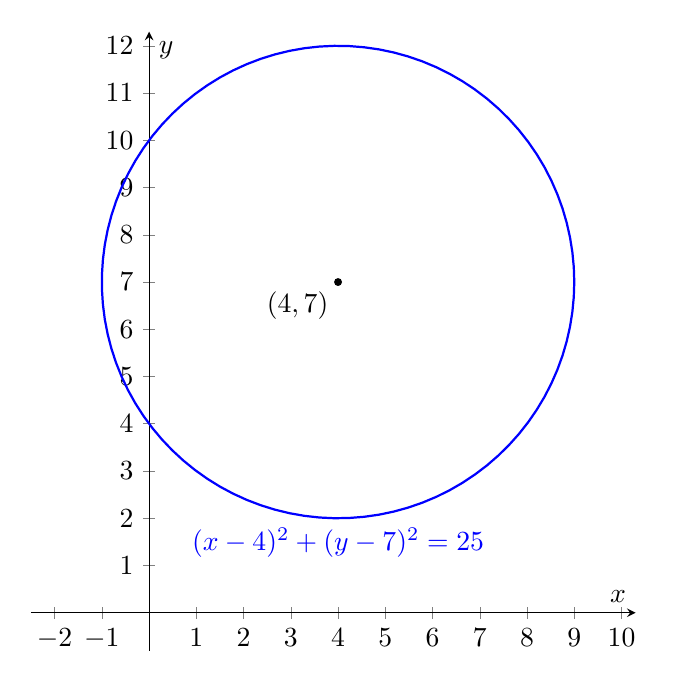
\begin{tikzpicture}
                   \begin{axis}[
x =0.6 cm, y=0.6 cm,
axis lines=middle,
xmin=-2.5,xmax=10.3,
ymin=-0.8,ymax=12.3,
xtick distance=1,
ytick distance=1,
xlabel=$x$,
ylabel=$y$
]
\addplot[thick, blue, domain=0:360, samples=100] ({4+5*cos(x)}, {7+5*sin(x)});
\node at (axis cs:4,7) [anchor=north east] {$(4,7)$};
\draw [fill=black, thick] (axis cs:4,7) circle (1pt);
\node at (axis cs:4,2) [blue, anchor=north] {$(x-4)^2+(y-7)^2=25$};
\end{axis}
                \end{tikzpicture}
            \end{center}
            Sedangkan, untuk sketsa grafik separuh lingkaran yang diberikan dalam soal, yaitu $x=4+\sqrt{-y^2+14y-24}$, merupakan bagian kanan dari lingkaran, yaitu sebagai berikut:
            \begin{center}
                \begin{tikzpicture}
                   \begin{axis}[
x =0.6 cm, y=0.6 cm,
axis lines=middle,
xmin=-2.5,xmax=10.3,
ymin=-0.8,ymax=12.3,
xtick distance=1,
ytick distance=1,
xlabel=$x$,
ylabel=$y$
]
\addplot[thick, blue, domain=-90:90, samples=100] ({4+5*cos(x)}, {7+5*sin(x)});
\end{axis}
                \end{tikzpicture}
            \end{center}
            \end{enumerate}}
        
    \end{jawab}
    \item Diketahui fungsi $f(x)=\left(\frac{3}{x}+x^2\right)^{3/2}$. Dapatkan $f'(2)$.\\
    \begin{jawab}[turunan fungsi, aturan rantai]{~\\
        Ingat kembali aturan rantai untuk turunan fungsi, yaitu
        \[
        \colorlet{oldcolor}{.}
        \color{blue}
        \setlength{\fboxrule}{1pt} \boxed{\color{oldcolor}\frac{d}{dx}[f(g(x))] = f'(g(x)) \cdot g'(x)}\color{oldcolor}.
        \]
        Dapat dimisalkan $\colorlet{oldcolor}{.}
        \color{blue}
        \setlength{\fboxrule}{1pt} \boxed{\color{oldcolor}u=g(x) = \frac{3}{x}+x^2}\color{oldcolor}$ sehingga $\colorlet{oldcolor}{.}
        \color{blue}
        \setlength{\fboxrule}{1pt} \boxed{\color{oldcolor}f(u) = u^{3/2}}\color{oldcolor}$, dan diperoleh
        \begin{align*}
            \colorlet{oldcolor}{.}
        \color{blue}
        \setlength{\fboxrule}{1pt} \boxed{\color{oldcolor}f'(u) = \frac{3}{2}u^{1/2}}\color{oldcolor} \quad \text{dan}\quad 
        \colorlet{oldcolor}{.}
        \color{blue}
        \setlength{\fboxrule}{1pt} \boxed{\color{oldcolor}g'(x) = -\frac{3}{x^2}+2x}\color{oldcolor}.
        \end{align*}
        Dengan demikian, diperoleh
        \begin{align*}
            f'(x) &= 
            f'(u) \cdot g'(x)\\
            &= \frac{3}{2}u^{1/2} \cdot \left(-\frac{3}{x^2}+2x\right)\\
            &= \frac{3}{2}\left(\frac{3}{x}+x^2\right)^{1/2} \left(-\frac{3}{x^2}+2x\right)\\
            &= \colorlet{oldcolor}{.}
        \color{blue}
        \setlength{\fboxrule}{1pt} \boxed{\color{oldcolor}\frac{3}{2}\left(\frac{3}{x}+x^2\right)^{1/2} \left(2x-\frac{3}{x^2}\right)}\color{oldcolor}.
        \end{align*}
        Selanjutnya, substitusi $x=2$ ke dalam $f'(x)$, diperoleh
        \begin{align*}
            f'(2) &= \frac{3}{2}\left(\frac{3}{2}+4\right)^{1/2} \left(4-\frac{3}{4}\right)\\
            &= \frac{3}{2}\left(\frac{11}{2}\right)^{1/2} \left(\frac{13}{4}\right)\\
            &= \colorlet{oldcolor}{.}
        \color{red}
        \setlength{\fboxrule}{1pt} \boxed{\color{oldcolor}\frac{39}{8}\sqrt{\frac{11}{2}}}\color{oldcolor}.
        \end{align*}
    }
    \end{jawab}
    \item Diberikan $f(x)=\begin{cases}
        \frac{\sqrt{x+9}-3}{x}, &x\neq 0\\
        \frac{1}{3}k-\frac{1}{5}, &x=0,
    \end{cases}, \text{dengan } x\in [-9,\infty)$.\\
    Tentukan nilai $k$ sehingga $\displaystyle\lim_{x\to 0}f(x)=f(0)$.\\
    Kemudian nyatakan fungsi $f(x)$ tanpa menggunakan bentuk fungsi sepotong-sepotong dalam domainnya untuk nilai $k$ yang diperoleh.\\
    \begin{jawab}[limit fungsi, fungsi kontinu, fungsi sepotong-sepotong]{~~\\
            Diperhatikan bahwa untuk \(x = 0\), $\colorlet{oldcolor}{.}
        \color{blue}
        \setlength{\fboxrule}{1pt} \boxed{\color{oldcolor}f(0) = \frac{1}{3}k-\frac{1}{5}}\color{oldcolor}$. Karena limit di $x=0$ artinya nilai fungsi di sekitar $x=0$ tetapi $x\neq 0$, didapatkan limitnya adalah
            \begin{align*}
            \lim_{x \to 0} f(x) = \lim_{x \to 0} \frac{\sqrt{x+9}-3}{x}.
            \end{align*}
            Untuk menyelesaikan limit tersebut, kita kalikan dengan bentuk konjugat (sekawan) dari pembilangnya, sehingga diperoleh
            \begin{align*}
                \lim_{x\to 0} f(x)&=\lim_{x\to 0}\frac{\sqrt{x+9}-3}{x}\cdot\frac{\sqrt{x+9}+3}{\sqrt{x+9}+3}\\
                &=\lim_{x\to 0}\frac{x+9-9}{x(\sqrt{x+9}+3)}\\
                &=\lim_{x\to 0}\frac{x}{x(\sqrt{x+9}+3)}\\
                &=\lim_{x\to 0}\frac{1}{\sqrt{x+9}+3}\\
                &=\colorlet{oldcolor}{.}
        \color{blue}
        \setlength{\fboxrule}{1pt} \boxed{\color{oldcolor}\frac{1}{6}}\color{oldcolor}.
            \end{align*}
            Karena $\displaystyle\lim_{x \to 0} f(x) = f(0)$, diperoleh
            \begin{align*}
                \frac{1}{6} = \frac{1}{3}k-\frac{1}{5} \implies \frac{1}{3}k = \frac{1}{6} + \frac{1}{5} = \frac{5+6}{30} = \frac{11}{30} \implies k = \frac{11}{30} \cdot 3 = \frac{11}{10}.
            \end{align*}
            Jadi nilai $k$ yang membuat $\lim_{x \to 0} f(x) = f(0)$ adalah $\colorlet{oldcolor}{.}
        \color{blue}
        \setlength{\fboxrule}{1pt} \boxed{\color{oldcolor}k = \frac{11}{10}}\color{oldcolor}$.
        Selanjutnya, untuk menyatakan fungsi $f(x)$ tanpa menggunakan bentuk fungsi sepotong-sepotong, kita dapat ambil ekspresi terakhir dari limit tersebut, yaitu
        \begin{align*}
            \colorlet{oldcolor}{.}
        \color{red}
        \setlength{\fboxrule}{1pt} \boxed{\color{oldcolor}f(x) = \frac{1}{\sqrt{x+9}+3}, \quad x \in [-9,\infty).}
        \end{align*}
    }
    \end{jawab}
\end{enumerate}
\newpage
 \begin{center}
	{\underline{\textbf{\MakeUppercase{Soal dan Pembahasan ETS Kalkulus 1 Tahun 2025/2026}}}}
    \end{center}

    \begin{center}
	\begin{tabular}{lcl}
		Mata kuliah/SKS & : & Kalkulus 1 ( SM234101 ) / 3 SKS\\
		Hari, Tanggal & : & Senin, 13 Oktober 2025\\
		Jam/Waktu Ujian & : & 13.30 - 15.10 / 100 menit\\
		Sifat & : & Tertutup\\
		Kelas & : & 13-16, 50-61\\
  ~
	\end{tabular}
    
    \noindent\rule{\textwidth}{2.pt}
        \end{center}
        \begin{enumerate}
            \item \begin{enumerate}
                \item Definisikan $|3-x|$.
                \item Berdasarkan point (a) tersebut, tentukan semua nilai $x$ yang memenuhi pertidaksamaan 
                \begin{align*}
                    |3-x|\leq -2x+1.
                \end{align*}
            \end{enumerate}
            \begin{jawab}[definisi nilai mutlak, pertidaksamaan nilai mutlak]{
                \begin{enumerate}
                    \item Ingat kembali definisi nilai mutlak, yaitu
                    \begin{align*}
                        |3-x| &= \begin{cases}
                            3-x, & 3-x \geq 0\\
                            -(3-x), & 3-x < 0
                        \end{cases} \\
                        &= \begin{cases}
                            3-x, & x\leq 3\\
                            x-3, & x>3
                        \end{cases}.
                    \end{align*}
                    \item Berdasarkan definisi tersebut, pertidaksamaan $|3-x|\leq -2x+1$ dapat ditulis menjadi dua kasus:
                    \begin{enumerate}
                        \item Jika $x\leq 3$, maka pertidaksamaan menjadi $3-x\leq -2x+1$, yang dapat diselesaikan menjadi $x\leq -2$.
                        \item Jika $x>3$, maka pertidaksamaan menjadi $x-3\leq -2x+1$, yang dapat diselesaikan menjadi $x\leq \frac{4}{3}$. Namun, karena kita berada pada kasus $x>3$, tidak ada solusi pada kasus ini.
                    \end{enumerate}
                    Jadi semua nilai $x$ yang memenuhi pertidaksamaan tersebut adalah $\colorlet{oldcolor}{.}
        \color{red}
        \setlength{\fboxrule}{1pt} \boxed{\color{oldcolor}x \leq 2}\color{oldcolor}$.
                \end{enumerate}
            }
                
            \end{jawab}
            \item 
            \begin{enumerate}
                \item Tentukan jarak titik $(1,3)$ dan $(7,11)$.
            \item Tentukan persamaan lingkaran yang diameternya adalah jarak titik $(1,3)$ ke $(7,11)$.
            \end{enumerate}
            \begin{jawab}[jarak titik, persamaan lingkaran]{
                \begin{enumerate}
                    \item Ingat kembali rumus jarak antara dua titik $(x_1,y_1)$ dan $(x_2,y_2)$, yaitu
                    \begin{align*}
                        d = \sqrt{(x_2-x_1)^2+(y_2-y_1)^2}.
                    \end{align*}
                    Dengan substitusi $(x_1,y_1)=(1,3)$ dan $(x_2,y_2)=(7,11)$, diperoleh
                    \begin{align*}
                        d &= \sqrt{(7-1)^2+(11-3)^2}\\
                        &= \sqrt{6^2+8^2}\\
                        &= \sqrt{36+64}\\
                        &= \sqrt{100}\\
                        &= 10.
                    \end{align*}
                    Jadi jarak antara titik $(1,3)$ dan $(7,11)$ adalah $\colorlet{oldcolor}{.}
        \color{red}
        \setlength{\fboxrule}{1pt} \boxed{\color{oldcolor}d = 10}\color{oldcolor}$.
                    \item Diketahui bahwa diameter lingkaran adalah jarak antara titik $(1,3)$ dan $(7,11)$, sehingga jari-jari lingkaran adalah setengah dari diameter, yaitu
                    \begin{align*}
                        r = \frac{d}{2} = \frac{10}{2} = 5.
                    \end{align*}
                    Karena diameternya berada di antara dua titik, maka pusat lingkaran adalah titik tengah dari dua titik tersebut. Titik tengah $(a,b)$ dari dua titik $(x_1,y_1)$ dan $(x_2,y_2)$ adalah
                    \begin{align*}
                        (a,b) = \left(\frac{x_1+x_2}{2},\frac{y_1+y_2}{2}\right).
                    \end{align*}
                    Dengan substitusi $(x_1,y_1)=(1,3)$ dan $(x_2,y_2)=(7,11)$, diperoleh
                    \begin{align*}
                        (a,b) = \left(\frac{1+7}{2}, \frac{3+11}{2}\right) = \left(\frac{8}{2}, \frac{14}{2}\right) = (4,7).
                    \end{align*}
                    Jadi pusat lingkaran adalah $(4,7)$ dan jari-jarinya adalah $5$. Persamaan lingkaran dengan pusat $(a,b)$ dan jari-jari $r$ adalah
                    \begin{align*}
                        (x-a)^2 + (y-b)^2 = r^2.
                    \end{align*}
                    Dengan substitusi $(a,b)=(4,7)$ dan $r=5$, diperoleh
                    \begin{align*}
                        (x-4)^2 + (y-7)^2 = 5^2 = 25
                    \end{align*}
                    Jadi persamaan lingkaran yang diameternya adalah jarak titik $(1,3)$ ke $(7,11)$ adalah $$\colorlet{oldcolor}{.}
        \color{red}
        \setlength{\fboxrule}{1pt} \boxed{\color{oldcolor}(x-4)^2 + (y-7)^2 = 25}\color{oldcolor}.$$
                \end{enumerate}
            }
            \end{jawab}
            \item Diberikan fungsi $f(x)=\begin{cases}
                x-1, &x<3\\
                2(x-4)^2, &x\geq 3
            \end{cases}$.
            \begin{enumerate}
                \item Dapatkan $f(3)$, $f(-2)$, dan $f(1-x^2)$.
                \item Dapatkan domain dan range dari $f(x)$.
                \item Sketsa grafik dari $f(x)$.
            \end{enumerate}
            \begin{jawab}[fungsi sepotong-sepotong, domain dan range fungsi, sketsa grafik]{
                \begin{enumerate}
                    \item Diperoleh
                    \begin{align*}
                        f(3) &= 2(3-4)^2 = 2(-1)^2 = 2\\
                        f(-2) &= -2-1 = -3\\
                        f(1-x^2) &= (1-x^2)-1 = -x^2.
                    \end{align*}
                    Jadi diperoleh $\colorlet{oldcolor}{.}
        \color{red}
        \setlength{\fboxrule}{1pt} \boxed{\color{oldcolor}f(3)=2,~f(-2)=-3,~f(1-x^2)=-x^2}\color{oldcolor}$.
                    \item Untuk $x<3$, $f(x)=x-1$ adalah fungsi linear dengan domain $(-\infty,3)$ dan range $(-\infty,2)$. Untuk $x\geq 3$, $f(x)=2(x-4)^2$ adalah fungsi kuadrat dengan domain $[3,\infty)$ dan range $[0,\infty)$. Dengan demikian, domain dari $f(x)$ adalah $\colorlet{oldcolor}{.}
        \color{red}
        \setlength{\fboxrule}{1pt} \boxed{\color{oldcolor}D(f)=(-\infty,3)\cup[3,\infty) = \mathbb{R}}\color{oldcolor}$, dan range dari $f(x)$ adalah $\colorlet{oldcolor}{.}
        \color{red}
        \setlength{\fboxrule}{1pt} \boxed{\color{oldcolor}R(f)=(-\infty,2)\cup[0,\infty) = (-\infty,2)\cup[0,\infty)}\color{oldcolor}$.
                    \item Sketsa grafik dari $f(x)$ adalah sebagai berikut:
                    % \begin{center}
                    %     \begin{tikzpicture}
                    %         \begin{axis}[
                    %             axis lines=middle,
                    %             xmin=-5, xmax=7,
                    %             ymin=-5, ymax=5,
                    %             xtick distance=1,
                    %             ytick distance=1,
                    %             xlabel=$x$,
                    %             ylabel=$f(x)$
                    %         ]
                    %         % Plot for x < 3
                    %         \addplot[domain=-5:3, thick, blue] {x-1};
                    %         % Plot for x >= 3
                    %         \addplot[domain=3:7, thick, red] {2*(x-4)^2};
                    %         % Mark the point at x=3
                    %         \addplot[only marks, mark=*] coordinates {(3,2)};
                    %         \end{axis}
                    %     \end{tikzpicture}
                    % \end{center}
                \end{enumerate}
            }   
                
            \end{jawab}
            \item Diberikan $f(x)=\frac{x^3-1}{x-1}$.
            \begin{enumerate}
                \item Tentukan $\displaystyle\lim_{x\to 1}f(x)$.
                \item Buatlah sketsa grafik $y=f(x)$.
            \end{enumerate}
            \begin{jawab}[limit fungsi, sketsa grafik]{
                \begin{enumerate}
                    \item Diperhatikan bahwa jika kita substitusi $x=1$ ke dalam $f(x)$, maka diperoleh bentuk tak tentu $\frac{0}{0}$. Oleh karena itu, kita faktorkan pembilangnya:
                    \begin{align*}
                        x^3-1 = (x-1)(x^2+x+1).
                    \end{align*}
                    Dengan demikian, fungsi dapat disederhanakan menjadi
                    \begin{align*}
                        f(x) = \frac{x^3-1}{x-1} = \frac{(x-1)(x^2+x+1)}{x-1} = x^2+x+1, \quad x\neq 1.
                    \end{align*}
                    Sekarang kita dapat menghitung limitnya:
                    \begin{align*}
                        \lim_{x\to 1}f(x) &= \lim_{x\to 1}(x^2+x+1)\\
                        &= 1^2 + 1 + 1\\
                        &= 3.
                    \end{align*}
                    Jadi $\colorlet{oldcolor}{.}
        \color{red}
        \setlength{\fboxrule}{1pt} \boxed{\color{oldcolor}\lim_{x\to 1}f(x) = 3}\color{oldcolor}$.
                    \item Sketsa grafik dari $y=f(x)$ adalah sebagai berikut:
                    % \begin{center}
                    %     \begin{tikzpicture}
                    %         \begin{axis}[
                    %             axis lines=middle,
                    %             xmin=-2, xmax=4,  
                   %             ymin=-1, ymax=5,
                    %             xtick distance=1,
                    %             ytick distance=1,
                    %             xlabel=$x$,
                    %             ylabel=$f(x)$
                    %         ]
                    %         \addplot[domain=-2:4, thick, blue] {x^2+x+1};
                    %         \addplot[only marks, mark=*] coordinates {(1,3)};
                    %         \end{axis}
                    %     \end{tikzpicture}
                    % \end{center}
                \end{enumerate}
            }
                
            \end{jawab}
            \item Diketahui kurva $x^2y+4x-3y^2=2$.
            \begin{enumerate}
                \item Dapatkan $\frac{dy}{dx}$ dengan menggunakan turunan fungsi implisit.
                \item Dari (a) dapatkan persamaan garis singgung pada kurva tersebut di titik $(1,1)$.
            \end{enumerate}
            \begin{jawab}[turunan implisit, persamaan garis singgung]{
                \begin{enumerate}
                    \item Kita turunkan kedua sisi persamaan $x^2y+4x-3y^2=2$ terhadap $x$, dengan mengingat bahwa $y$ adalah fungsi dari $x$ (yaitu $y=y(x)$):
                    \begin{align*}
                        \frac{d}{dx}(x^2y) + \frac{d}{dx}(4x) - \frac{d}{dx}(3y^2) &= \frac{d}{dx}(2)\\
                        2xy + x^2\frac{dy}{dx} + 4 - 6y\frac{dy}{dx} &= 0.
                    \end{align*}
                    Sekarang kita kumpulkan semua suku yang mengandung $\frac{dy}{dx}$ di satu sisi:
                    \begin{align*}
                        x^2\frac{dy}{dx} - 6y\frac{dy}{dx} &= -2xy - 4\\
                        (x^2 - 6y)\frac{dy}{dx} &= -2xy - 4\\
                        \frac{dy}{dx} &= \frac{-2xy - 4}{x^2 - 6y}.
                    \end{align*}
                    Jadi diperoleh $\colorlet{oldcolor}{.}
        \color{red}
        \setlength{\fboxrule}{1pt} \boxed{\color{oldcolor}\frac{dy}{dx} = \frac{-2xy - 4}{x^2 - 6y}}\color{oldcolor}$.
                    \item Untuk mendapatkan persamaan garis singgung di titik $(1,1)$, kita substitusi $x=1$ dan $y=1$ ke dalam turunan yang telah kita peroleh:
                    \begin{align*}
                        \left.\frac{dy}{dx}\right|_{(1,1)} &= \frac{-2(1)(1) - 4}{(1)^2 - 6(1)}\\
                        &= \frac{-2 - 4}{1 - 6}\\
                        &= \frac{-6}{-5}\\
                        &= \frac{6}{5}.
                    \end{align*}
                    Jadi kemiringan garis singgung di titik $(1,1)$ adalah $\frac{6}{5}$. Dengan menggunakan persamaan garis singgung $y - y_1 = m(x - x_1)$, di mana $(x_1,y_1)=(1,1)$ dan $m=\frac{6}{5}$, diperoleh:
                    \begin{align*}
                        y - 1 &= \frac{6}{5}(x - 1)\\
                        y - 1 &= \frac{6}{5}x - \frac{6}{5}\\
                        y &= \frac{6}{5}x - \frac{6}{5} + 1\\
                        y &= \frac{6}{5}x - \frac{6}{5} + \frac{5}{5}\\
                        y &= \frac{6}{5}x - \frac{1}{5}.
                    \end{align*}
                    Jadi persamaan garis singgung di titik $(1,1)$ adalah $\colorlet{oldcolor}{.}
        \color{red}
        \setlength{\fboxrule}{1pt} \boxed{\color{oldcolor}y = \frac{6}{5}x - \frac{1}{5}}\color{oldcolor}$.
                \end{enumerate}
            }
                
            \end{jawab}
        \end{enumerate}
\newpage
 \begin{center}
	{\underline{\textbf{\MakeUppercase{Soal dan Pembahasan ETS Kalkulus 1 Tahun 2025/2026}}}}
    \end{center}

    \begin{center}
	\begin{tabular}{lcl}
		Mata kuliah/SKS & : & Kalkulus 1 ( SM234101 ) / 3 SKS\\
		Hari, Tanggal & : & Selasa, 14 Oktober 2025\\
		Waktu & : & 07.00 - 08.40 / 100 menit\\
		Sifat & : & Tertutup\\
		Kelas & : & 113 dan 114\\
  ~
	\end{tabular}
    
    \noindent\rule{\textwidth}{2.pt}
        \end{center}
        \begin{enumerate}
            \item Dapatkan penyelesaian dari pertidaksamaan 
            \begin{align*}
                \frac{x^2-x-12}{x^2+3x-10}\geq 0.
            \end{align*}
            \begin{jawab}[pertidaksamaan rasional, faktorisasi, garis bilangan]{
                Pertama, kita faktorkan pembilang dan penyebut:
                \begin{align*}
                    x^2 - x - 12 &= (x-4)(x+3),\\
                    x^2 + 3x - 10 &= (x+5)(x-2).
                \end{align*}
                Jadi pertidaksamaan menjadi:
                \begin{align*}
                    \frac{(x-4)(x+3)}{(x+5)(x-2)} \geq 0.
                \end{align*}
                Didapatkan pembuat nol dari pembilang adalah $x=4$ dan $x=-3$, dan pembuat nol dari penyebut adalah $x=-5$ dan $x=2$. Selanjutnya, dibuat garis bilangan dan tentukan tanda dari setiap interval:
                \begin{itemize}
                    \item Interval $(-\infty, -5)$: Pilih $x=-6$, maka $\frac{(-)(-)}{(-)(-)} = \frac{(+)(+)}{(+)(+)} > 0$.
                    \item Interval $(-5, -3)$: Pilih $x=-4$, maka $\frac{(-)(-)}{(+)(-)} = \frac{(+)(+)}{(-)(-)} < 0$.
                    \item Interval $(-3, 2)$: Pilih $x=0$, maka $\frac{(-)(+)}{(+)(-)} = \frac{(-)(+)}{(+)(-)} > 0$.
                    \item Interval $(2, 4)$: Pilih $x=3$, maka $\frac{(-)(+)}{(+)(+)} = \frac{(-)(+)}{(+)(+)} < 0$.
                    \item Interval $(4, \infty)$: Pilih $x=5$, maka $\frac{(+)(+)}{(+)(+)} = \frac{(+)(+)}{(+)(+)} > 0$.
                \end{itemize}
                Jadi tanda dari setiap interval adalah:
                \begin{align*}
                    (-\infty, -5): +, \quad (-5, -3): -, \quad (-3, 2): +, \quad (2, 4): -, \quad (4, \infty): +.
                \end{align*}
                Karena kita mencari di mana ekspresi tersebut $\geq 0$, kita ambil interval di mana tanda positif dan juga titik-titik di mana pembilangnya nol (yaitu $x=-3$ dan $x=4$). Namun, kita tidak termasuk titik-titik di mana penyebutnya nol (yaitu $x=-5$ dan $x=2$) karena itu akan membuat ekspresi tidak terdefinisi. Jadi solusi dari pertidaksamaan adalah:
                \begin{align*}
                    x \in (-\infty, -5) \cup [-3, 2) \cup [4, \infty).
                \end{align*}
                Jadi penyelesaian dari pertidaksamaan tersebut adalah $\colorlet{oldcolor}{.}
        \color{red}
        \setlength{\fboxrule}{1pt} \boxed{\color{oldcolor}x \in (-\infty, -5) \cup [-3, 2) \cup [4, \infty)}\color{oldcolor}$.
            }
                
            \end{jawab}
            \item \begin{enumerate}
                \item Dapatkan kemiringan garis $\ell$ yang melalui titik $(0,0)$ dan $(-2,1)$.
                \item Jika garis $\ell$ tegak lurus dengan garis yang menyinggung lingkaran yang berpusat di $(0,0)$ dan berjari-jari $\sqrt{5}$, di titik $(-2,1)$, maka dapatkan persamaan garis singgung lingkaran tersebut dan sketsalah.
            \end{enumerate}
            \begin{jawab}[kemiringan garis, garis singgung lingkaran]{
                \begin{enumerate}
                    \item Kemiringan garis yang melalui dua titik $(x_1,y_1)$ dan $(x_2,y_2)$ adalah
                    \begin{align*}
                        m = \frac{y_2 - y_1}{x_2 - x_1}.
                    \end{align*}
                    Dengan substitusi $(x_1,y_1)=(0,0)$ dan $(x_2,y_2)=(-2,1)$, diperoleh
                    \begin{align*}
                        m &= \frac{1 - 0}{-2 - 0} = \frac{1}{-2} = -\frac{1}{2}.
                    \end{align*}
                    Jadi kemiringan garis $\ell$ adalah $\colorlet{oldcolor}{.}
        \color{red}
        \setlength{\fboxrule}{1pt} \boxed{\color{oldcolor}m = -\frac{1}{2}}\color{oldcolor}$.
                    \item
                    Persamaan lingkaran yang berpusat di $(0,0)$ dan berjari-jari $\sqrt{5}$ adalah
                    \begin{align*}
                        x^2 + y^2 = 5.
                    \end{align*}
                    Untuk mendapatkan garis singgung di titik $(-2,1)$, kita pertama-tama perlu memastikan bahwa titik tersebut berada pada lingkaran. Substitusi $(-2,1)$ ke dalam persamaan lingkaran:
                    \begin{align*}
                        (-2)^2 + (1)^2 = 4 + 1 = 5,
                    \end{align*}
                    yang sesuai dengan persamaan lingkaran, jadi titik tersebut memang berada pada lingkaran.
                    Kemiringan garis singgung pada lingkaran di titik $(x_0,y_0)$ dapat diperoleh dari fakta bahwa garis singgungnya tegak lurus dengan garis $\ell$ yang melalui pusat lingkaran dan titik tersebut. Garis dari pusat $(0,0)$ ke titik $(-2,1)$ memiliki kemiringan
                    \begin{align*}
                        m_{radius} = \frac{1 - 0}{-2 - 0} = \frac{1}{-2} = -\frac{1}{2}.
                    \end{align*}
                    \end{enumerate}
            }
                \end{jawab}
            \item Tuliskan rumus turunan dari $fg$ yaitu $\frac{d}{dx}(f(x)g(x))$\\
            Selanjutnya, dapatkan turunan dari $fg$, jika diketahui $f(x)=3x^2-7x$ dan $g(x)=3-2x^2$.
            \item Dapatkan $\displaystyle \lim_{x\to 3} \frac{\sqrt{3x+7}-4}{x-3}$.
            \item Diberikan fungsi $f(x)=\frac{1}{x-1}$ dan $g(x)=x^2$.
            \begin{enumerate}
                \item Dapatkan $(f\circ g)(x)$.
                \item Jika diketahui $(p\circ g)(x)=  x^2-3$, dapatkan $p(x)$.
            \end{enumerate}
        \end{enumerate}

\newpage
 \begin{center}
	{\underline{\textbf{\MakeUppercase{Soal dan Pembahasan ETS Kalkulus 1 Tahun 2025/2026}}}}
    \end{center}

    \begin{center}
	\begin{tabular}{lcl}
		Course / Credit & : & Kalkulus 1 ( SM234101 ) / 3 SKS\\
		Day, Date & : & Tuesday, 14 October 2025\\
		Time / Exam Time & : & 07.00 - 08.40 / 100 menit\\
		Type & : & Closed\\
		Class & : & 2, 3, 68, 69\\
  ~
	\end{tabular}
    
    \noindent\rule{\textwidth}{2.pt}
        \end{center}
        \begin{enumerate}
            \item Find the solution of the following inequality 
            \begin{align*}
                \frac{x^2-x-12}{x^2+3x-10}\geq 0.
            \end{align*}
            \item \begin{enumerate}
                \item Find the gradient of the line $\ell$ which goes through $(0,0)$ and $(-2,1)$.
                \item If line $\ell$ is perpendicular with the line that tangent with a circle centered at $(0,0)$ and radius $\sqrt{5}$, at $(-2,1)$, then find the aforementioned tangent line equation and sketch the graph. 
            \end{enumerate}
            \item Write the derivative formula of $fg$ that is $\frac{d}{dx}(f(x)g(x))$\\
            Then, find the derivative of $fg$, given that $f(x)=3x^2-7x$ and $g(x)=3-2x^2$.
            \item Calculate $\displaystyle \lim_{x\to 3} \frac{\sqrt{3x+7}-4}{x-3}$.
            \item Given a function $f(x)=\frac{1}{x-1}$ and $g(x)=x^2$. 
            \begin{enumerate}
                \item Find $(f\circ g)(x)$.
                \item Given $(p\circ g)(x)=  x^2-3$, then find $p(x)$.
            \end{enumerate}
        \end{enumerate}
               \newpage
 \begin{center}
	{\underline{\textbf{\MakeUppercase{Soal dan Pembahasan ETS Kalkulus 1 Tahun 2025/2026}}}}
    \end{center}

    \begin{center}
	\begin{tabular}{lcl}
		Mata kuliah/SKS & : & Kalkulus 1 ( SM234101 ) / 3 SKS\\
		Hari, Tanggal & : & Selasa, 14 Oktober 2025\\
		Waktu & : & 09.00 - 10.40 / 100 menit\\
		Sifat & : & Tertutup\\
		Kelas & : & 5-12, 23-29, 115 dan 116\\
  ~
	\end{tabular}
    
    \noindent\rule{\textwidth}{2.pt}
        \end{center}
        \begin{enumerate}
            \item Selesaikan pertidaksamaan berikut 
            \begin{align*}
                \frac{1}{x+2} \leq \frac{2}{x-1}.
            \end{align*}
            \item Gambarkan kurva dasar $y=\frac{1}{x}$. Berdasarkan kurva dasar tersebut, gunakan translasi (pergeseran) untuk menggambar kurva $y=\frac{1}{x-2}+4$ (Jelaskan ilustrasinya).
            \item Diberikan fungsi $f(x)=\frac{1}{x-2}$ dan $g(x)=\sqrt{5-x}$. Tentukan :
            \begin{enumerate}
                \item Domain fungsi $f$ dan $g$.
                \item Fungsi $(f\circ g)(x)$ dan $\left(\frac{f}{g}\right) (x)$ beserta domainnya masing-masing. 
            \end{enumerate}
            \item Tunjukkan bahwa $f(x)=\begin{cases}
                3x+1, &x\leq 2\\
                x+5, &x>2
            \end{cases}$ adalah fungsi kontinu tetapi tidak dapat diturunkan di $x=2$.
            \item Tentukan $\frac{dy}{dx}$ jika $x^2y+y^3=10$.
        \end{enumerate}
               \newpage
 \begin{center}
	{\underline{\textbf{\MakeUppercase{Soal dan Pembahasan ETS Kalkulus 1 Tahun 2025/2026}}}}
    \end{center}

    \begin{center}
	\begin{tabular}{lcl}
		Mata kuliah/SKS & : & Kalkulus 1 ( SM234101 ) / 3 SKS\\
		Hari, Tanggal & : & Selasa, 14 Oktober 2025\\
		Waktu & : & 11.00 - 12.40 / 100 menit\\
		Sifat & : & Tertutup\\
		Kelas & : & 102, 108-112\\
  ~
	\end{tabular}
    
    \noindent\rule{\textwidth}{2.pt}
        \end{center}
        \begin{enumerate}
            \item Dapatkan solusi dari ketaksamaan 
            \begin{align*}
                2<|3-x|\leq 5.
            \end{align*}
            Petunjuk: Gunakan rumus jarak.
            \item Diketahui garis $\ell_1$ dengan gradien $m_1=\frac{2}{3}$ dan garis $\ell_2$ berpotongan tegak lurus dengan $\ell_1$ di titik $(4,-1)$. Dapatkan persamaan garis $\ell_2$. \\
            Gambarkan kedua garis $\ell_1$ dan $\ell_2$ pada satu bidang koordinat. 
            \item Diketahui $f(x)=x^2-4x$.
            \begin{enumerate}
                \item Tentukan domain alami untuk $x$ agar $f(x)$ mempunyai invers.
                \item Dapatkan $f^{-1}(x)$, domain, dan rangenya. 
            \end{enumerate}
            \item Diberikan fungsi 
            \begin{align*}
                f(x)=\begin{cases}
                    \frac{x^2-9}{x+3}, &x\neq -3\\
                    k, &x=-3
                \end{cases}
            \end{align*}
            \begin{enumerate}
                \item Tentukan nilai $k$ agar $f(-3)=\displaystyle\lim_{x\to -3} f(x)$.
                \item Dengan memberi $k$ pada $\lim_{x\to-3} f(x)$, tunjukkan bahwa $f(x)$ dapat dinyatakan sebagai fungsi polinomial. 
            \end{enumerate}
            \item Diketahui $f(x)=(\sqrt{x}+2x^2+1)^5$.\\
            Dengan aturan rantai, dapatkan turunan pertama dari $f(x)$.
        \end{enumerate}
               \newpage
 \begin{center}
	{\underline{\textbf{\MakeUppercase{Soal dan Pembahasan ETS Kalkulus 1 Tahun 2025/2026}}}}
    \end{center}

    \begin{center}
	\begin{tabular}{lcl}
		Mata kuliah/SKS & : & Kalkulus 1 ( SM234101 ) / 3 SKS\\
		Hari, Tanggal & : & Selasa, 14 Oktober 2025\\
		Waktu & : & 15.30 - 17.10 / 100 menit\\
		Sifat & : & Tertutup\\
		Kelas & : & 30-39\\
  ~
	\end{tabular}
    
    \noindent\rule{\textwidth}{2.pt}
        \end{center}
        \begin{enumerate}
            \item Dapatkan penyelesaian dari pertidaksamaan 
            \begin{align*}
                2\leq x^2-2\leq 7.
            \end{align*}
            \item Gunakan grafik dasar $x=y^2$ dan sifat pergeseran/translasi untuk menggambar parabola $x=y^2+2y+3$.
            \item Tentukan domain dari fungsi $(f\circ g)(x)$ jika diketahui fungsi $g(x)=2x+3$ dengan $0\leq x<3$ dan fungsi $f$ terdefinisi pada interval $-1\leq x <5$.
            \item Diberikan fungsi $f(x)=\left|\frac{x^2-9}{x-3}\right|$. Dapatkan titik $x$ di mana membuat fungsi $f(x)$ diskontinu?\\
            Dapatkan nilai fungsi $f(x)$ pada titik tersebut agar menjadi kontinu dan sketsa grafik fungsi tersebut.
            \item Dengan diferensiasi implisit, dapatkan $\frac{dy}{dx}$ dari $x^3y^2-3xy^2+x=1$.
        \end{enumerate}
 \newpage
 \begin{center}
	{\underline{\textbf{\MakeUppercase{Soal dan Pembahasan ETS Matematika Tahun 2025/2026}}}}
    \end{center}

    \begin{center}
	\begin{tabular}{lcl}
		Mata kuliah/SKS & : & Matematika ( SM234152 ) / 2 SKS\\
		Hari, Tanggal & : & Jumat, 17 Oktober 2025\\
		Waktu & : & 07.00 - 08.40 / 100 menit\\
		Sifat & : & Tertutup\\
		Kelas & : & 1-8\
  ~
	\end{tabular}
    
    \noindent\rule{\textwidth}{2.pt}
        \end{center}
\begin{enumerate}
    \item Diberikan SPL 
    \begin{align*}
        x+y+2z &= 8\\
        -x-2y+3z &= 1\\
        3x-7y+4z &= 10
    \end{align*}
    \begin{enumerate}
        \item Nyatakan SPL tersebut dalam bentuk persamaan matriks $A\overline{x}=b$.
        \item Menggunakan Eliminasi Gauss, carilah solusi (jika ada) dari SPL tersebut.
    \end{enumerate}
    \item Carilah himpunan penyelesaian dari pertidaksamaan
    \begin{align*}
        1<|3x-4|\leq 6.
    \end{align*}
    \item Tentukan nilai $k$ agar garis $\ell_1:kx-3y=12$ tegak lurus dengan garis $\ell_2:2x+3y=6$.
    \item Selesaikan persamaan berikut 
    \begin{align*}
        \ln \left(\frac{1}{x}\right)+\ln(4x^3)=2.
    \end{align*}
    \item Diberikan sistem persamaan fungsi permintaan dan penawaran (\textit{supply and demand})
    \begin{align*}
       4P=-Q_d+93\\
       5P=Q_s+33
    \end{align*}
    dengan $P,Q_d,Q_s$ masing-masing adalah harga, jumlah permintaan (\textit{demand}), dan jumlah penawaran (\textit{supply}).
    \begin{enumerate}
        \item Jika harga barang $Rp5.000$, berapa jumlah unit permintaan>
        \item Jika jumlah barang yang ditawarkan 17 unit, berapa harga penawarannya.
        \item Tentukan harga dan jumlah barang di titik equilibrium.
        \item Gambarkan/sket kurva penawaran dan permintaan dan titik keseimbangannya.
    \end{enumerate}
\end{enumerate}
\newpage 

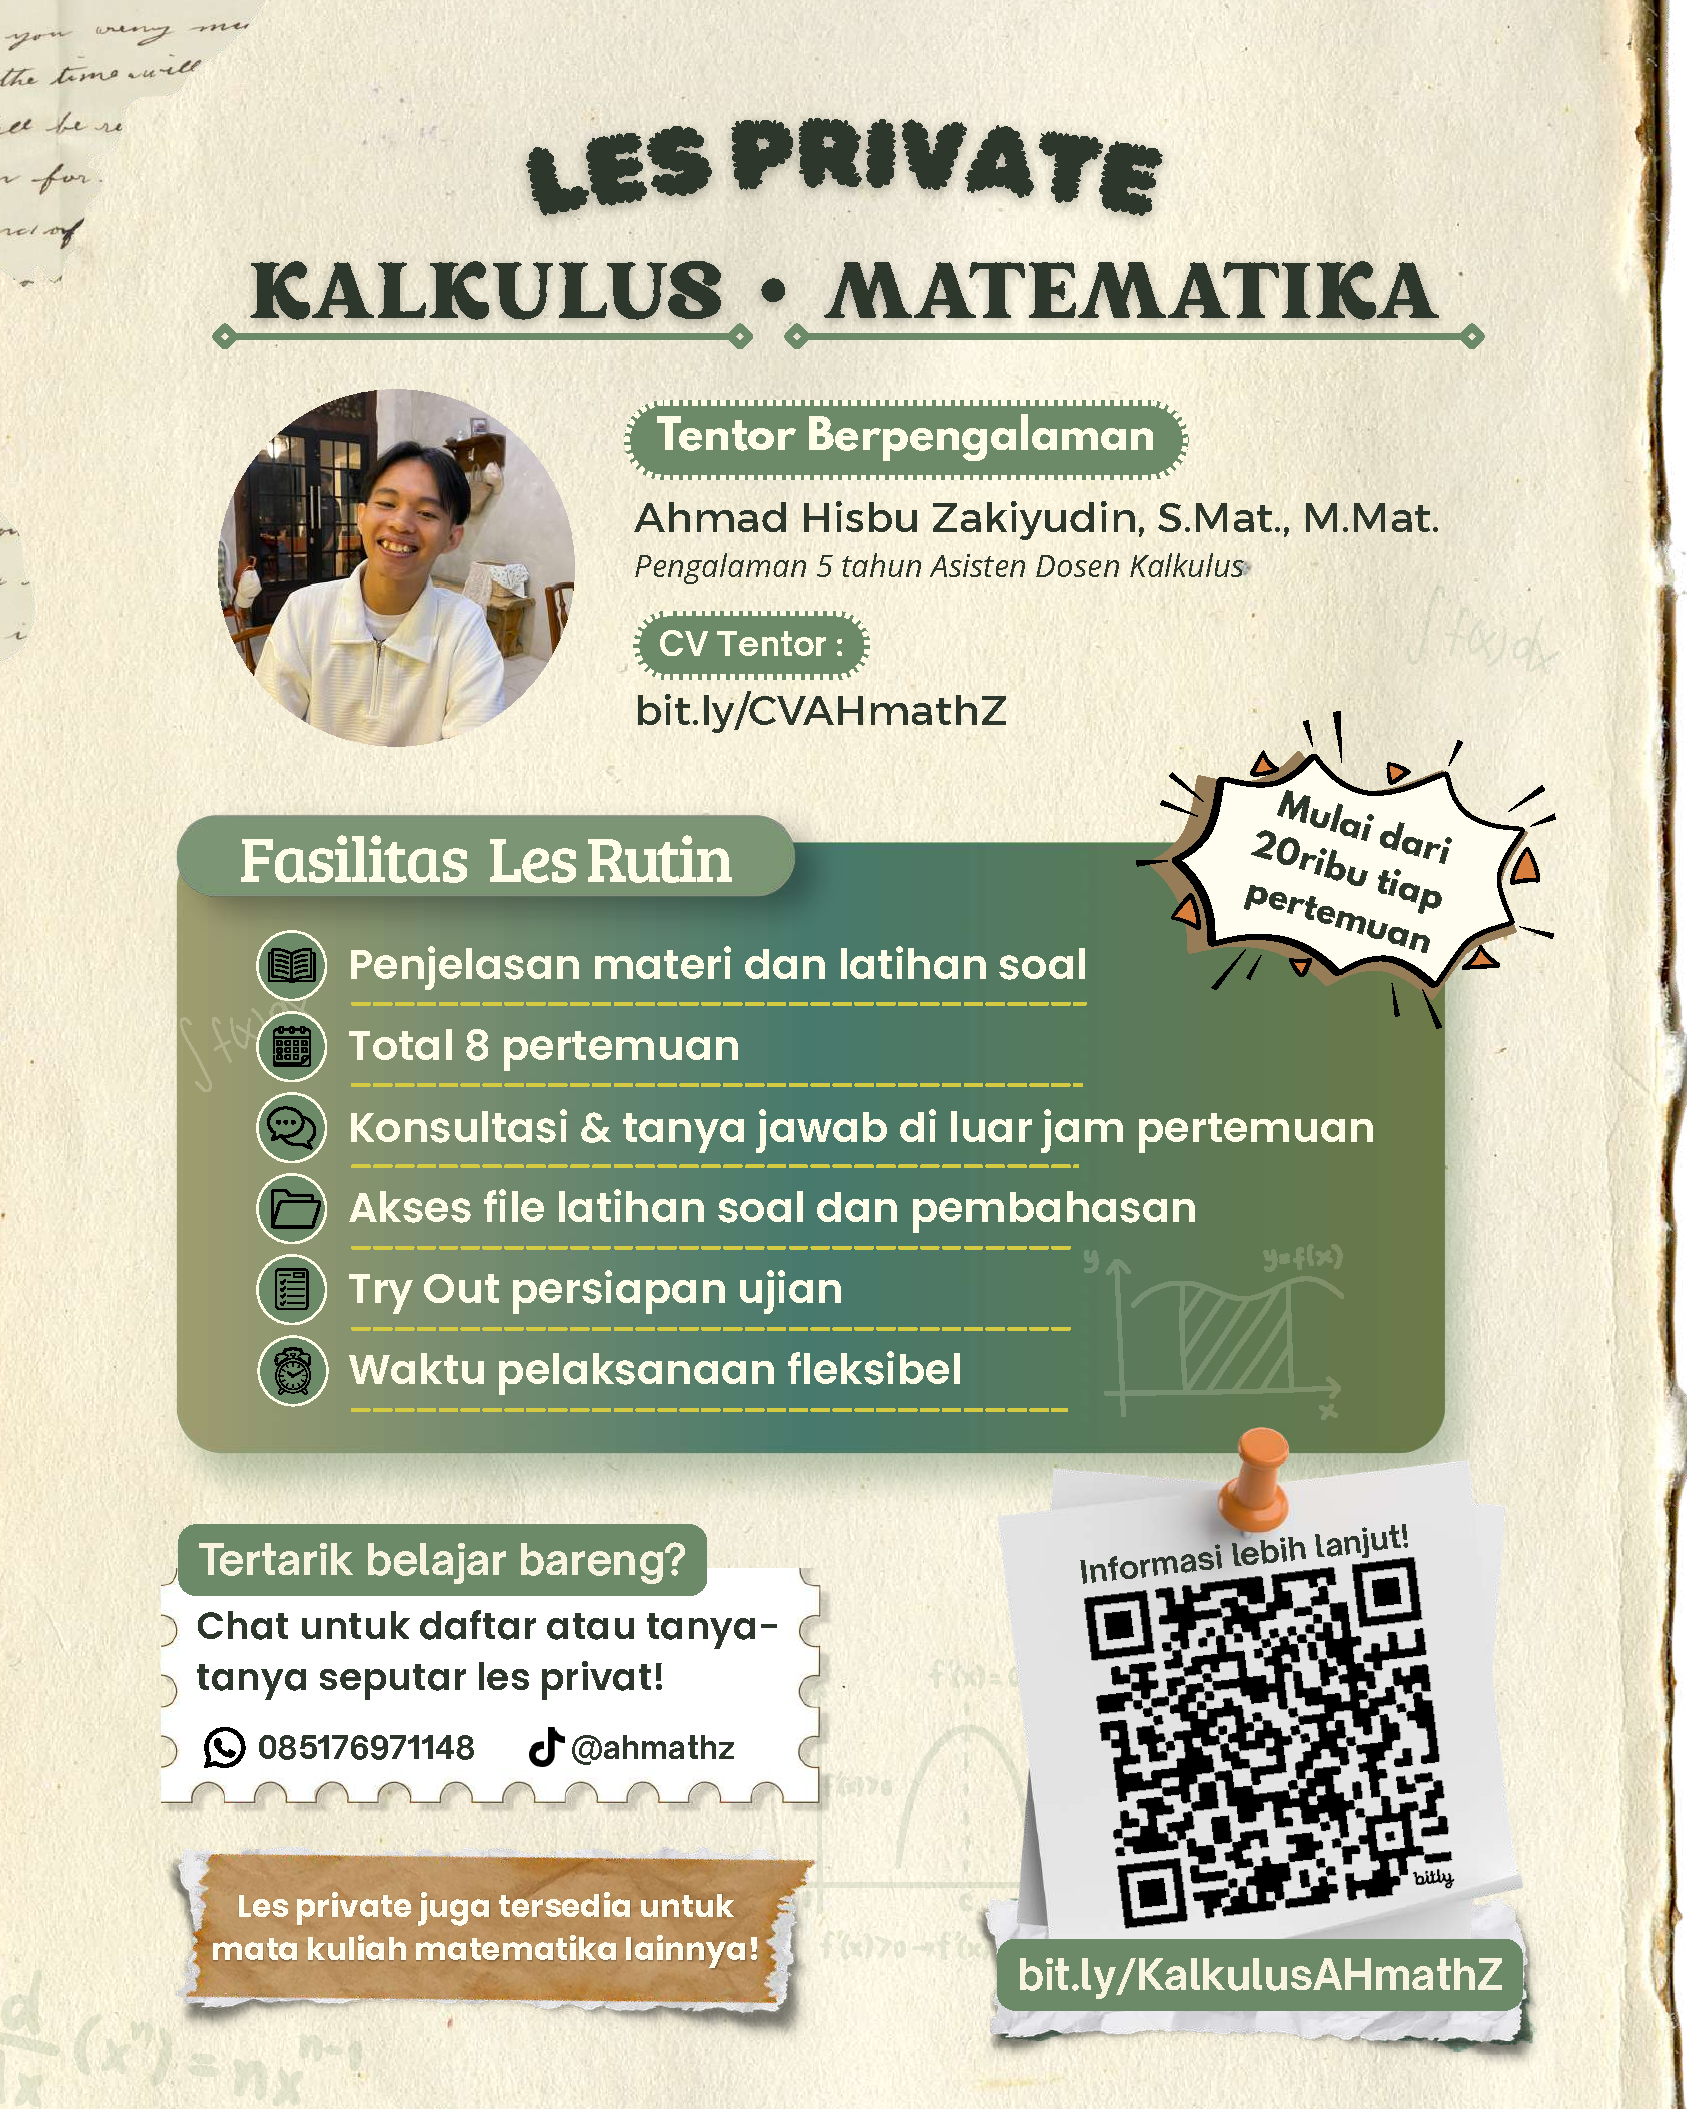
\includepdf[pages=-]{les.pdf}

\end{document}


